\documentclass[conference]{IEEEtran}
\IEEEoverridecommandlockouts
\usepackage{cite}
\usepackage{url}
\usepackage{amsmath,amssymb,amsfonts}
\usepackage{algorithm}
\usepackage{algpseudocode}
\usepackage{graphicx}
\usepackage{textcomp}
\usepackage[utf8]{inputenc}
\usepackage{xcolor}
\usepackage{amsfonts}
\usepackage{longtable}
\usepackage{tabularx}
\usepackage{subcaption}
\usepackage{geometry}
\usepackage{multirow}
\usepackage{booktabs}
\usepackage{tikz}
\usetikzlibrary{positioning,arrows.meta,shapes.geometric,fit,calc}
\geometry{top=0.7in, right=0.58in, left=0.58in, bottom=4.33cm}
\def\BibTeX{{\rm B\kern-.05em{\sc i\kern-.025em b}\kern-.08em
    T\kern-.1667em\lower.7ex\hbox{E}\kern-.125emX}}

\title{RALPH: Multi-Agent LLM-Augmented Bayesian Optimization for Statistically Rigorous Quantitative Strategy Discovery}

\author{
\IEEEauthorblockN{Lakshin Pathak}
\IEEEauthorblockA{Tatvic Analytics, Ahmedabad, India}
\IEEEauthorblockA{Email: lakshin@tatvic.com}
}

\begin{document}
\maketitle

% ═══════════════════════════════════════════════════════════════════════════════
\begin{abstract}
This paper presents \textbf{RALPH} (\textit{Robust Adaptive Learning in Portfolio Heuristics}), a multi-agent framework that integrates Bayesian optimization via Gaussian Process (GP) surrogates, walk-forward out-of-sample validation, and Large Language Model (LLM) intelligence layers for automated quantitative trading strategy discovery. The framework addresses critical challenges in algorithmic strategy development: data snooping bias from multiple hypothesis testing, high-dimensional hyperparameter optimization, and the absence of qualitative market context in purely mathematical pipelines. RALPH employs a seven-agent architecture where each agent handles a distinct stage --- sentiment analysis, signal generation, position sizing via Kelly criterion and GARCH(1,1) volatility, event-driven backtesting with Almgren-Chriss transaction costs, statistical validation, Deflated Sharpe Ratio (DSR) computation, and GP-based parameter mutation with LLM-guided exploration. Applied to Indian equity markets (RELIANCE.NS, NSE), the system demonstrates that combining mathematical rigor with structured LLM reasoning produces an auditable, interpretable, and statistically sound strategy evaluation pipeline. The framework achieves full automation from discovery to Google Sheets reporting at a cost of \$0.011 per iteration using Google Gemini 3 Flash, with graceful degradation when LLM services are unavailable.
\end{abstract}

\begin{IEEEkeywords}
Multi-Agent Systems, Quantitative Finance, Bayesian Optimization, Large Language Models, Deflated Sharpe Ratio, Walk-Forward Validation, Algorithmic Trading, Gaussian Process
\end{IEEEkeywords}

% ═══════════════════════════════════════════════════════════════════════════════
\section{Introduction}
\label{sec:introduction}

The quantitative finance industry is undergoing a transformative shift as machine learning techniques, high-frequency data sources, and increasingly sophisticated optimization algorithms converge to reshape how trading strategies are discovered, validated, and deployed. At the heart of this transformation lies a fundamental epistemological challenge: how can one reliably distinguish a genuinely profitable trading strategy from a statistical artifact produced by extensive backtesting? This question, long debated in academic finance, has become even more urgent as the democratization of financial data and computing power enables practitioners to evaluate thousands of parameter combinations on the same historical dataset in a matter of minutes \cite{harvey2016backtesting}.

The practice of repeatedly testing strategies on the same data --- commonly referred to as \textit{data snooping} or \textit{selection bias} --- systematically inflates performance metrics. A strategy that appears to generate a Sharpe ratio of 2.0 in-sample may, in fact, be entirely attributable to the law of large numbers: when hundreds of hypotheses are tested, some will inevitably produce impressive results by pure chance. Bailey and L\'{o}pez de Prado \cite{bailey2014deflated} formalized this insight through the Deflated Sharpe Ratio (DSR), demonstrating that the expected maximum Sharpe ratio among $N$ independent trials grows as $O(\sqrt{\log N})$ even when no strategy has any genuine predictive power. This finding has profound implications for the industry, where backtested track records routinely serve as the primary evidence for strategy viability.

Simultaneously, the emergence of Large Language Models (LLMs) such as GPT-4, Claude, and Google Gemini has created an unprecedented opportunity to bridge the gap between quantitative analysis and qualitative market understanding. Experienced portfolio managers naturally incorporate news sentiment, macroeconomic context, and regime awareness into their decisions --- capabilities that purely mathematical systems lack. Yet, integrating LLMs into financial decision-making pipelines raises critical concerns about reliability, hallucination risk, and the appropriate boundary between deterministic computation and probabilistic language generation.

This paper addresses these converging challenges through the design and implementation of RALPH (\textit{Robust Adaptive Learning in Portfolio Heuristics}), a multi-agent framework that brings together three pillars of modern quantitative research:

\begin{itemize}
    \item \textbf{Bayesian Optimization:} A Gaussian Process (GP) surrogate model enables sample-efficient exploration of the strategy parameter space, dramatically reducing the number of evaluations needed compared to grid search or random search.
    \item \textbf{Statistical Rigor:} The Deflated Sharpe Ratio is computed at \textit{every} iteration --- not merely as a post-hoc check --- ensuring that the multiple testing penalty is integrated into the optimization loop itself.
    \item \textbf{LLM Intelligence:} A structured LLM layer provides qualitative assessments, narrative explanations, and mutation guidance, while a strict architectural principle ensures that no trading decision ever depends on LLM output.
\end{itemize}

The remainder of this paper is organized as follows: Section II reviews the related literature across statistical testing, Bayesian optimization, and LLMs in finance. Section III formalizes the system model and problem formulation. Section IV details the seven-agent architecture and the RALPH loop. Section V presents experimental results on Indian equity markets. Section VI discusses findings, limitations, and future directions. Section VII concludes the paper.

% ═══════════════════════════════════════════════════════════════════════════════
\section{Related Work}
\label{sec:related}

\subsection{Statistical Corrections for Multiple Testing in Finance}
The problem of multiple hypothesis testing in backtesting was first rigorously addressed by Bailey and L\'{o}pez de Prado \cite{bailey2014deflated}, who introduced the Deflated Sharpe Ratio. Their work showed that the observed Sharpe ratio must be adjusted for the number of trials conducted, the non-normality of return distributions (measured by skewness and excess kurtosis), and the length of the track record. Without such corrections, a researcher testing 200 strategy variants should expect to find strategies with Sharpe ratios exceeding 1.5, even if all strategies are entirely random.

Harvey et al. \cite{harvey2016backtesting} extended this analysis to the academic literature on cross-sectional asset pricing anomalies. They demonstrated that the majority of published ``factors'' fail to survive proper multiple testing corrections and proposed raising the $t$-statistic threshold from the traditional 2.0 to 3.0 for any claimed discovery. This finding underscored the systemic nature of the problem and motivated frameworks like the Probability of Backtest Overfitting (PBO), introduced by Bailey et al. \cite{bailey2017probability}, which uses combinatorial cross-validation to estimate the likelihood that a backtested strategy is overfit to historical data.

RALPH integrates both DSR and a simplified PBO estimate as complementary metrics. The DSR serves as the primary selection criterion during optimization, while PBO provides an independent check on overfitting risk.

\subsection{Bayesian Optimization for Hyperparameter Tuning}
Bayesian optimization, formalized by Snoek et al. \cite{snoek2012practical}, has become the standard approach for sample-efficient optimization of expensive black-box functions in machine learning. The core idea is to model the unknown objective function as a sample from a Gaussian Process and use an acquisition function --- typically Expected Improvement (EI) or Upper Confidence Bound (UCB) --- to select the next evaluation point. This approach balances exploration of uncertain regions with exploitation of promising areas, achieving near-optimal solutions in far fewer evaluations than grid search.

In the financial domain, Gonz\'{a}lvez et al. \cite{gonzalvez2019financial} applied GP-based methods to portfolio optimization, demonstrating that Bayesian approaches outperform random search in both sample efficiency and final solution quality. However, their work focused on static portfolio weights rather than the dynamic, event-driven strategies that RALPH targets. RALPH extends the Bayesian optimization paradigm by coupling the GP surrogate with an LLM oracle capable of overriding GP suggestions based on qualitative reasoning, creating a hybrid human-AI exploration mechanism.

\subsection{Large Language Models in Financial Applications}
The application of LLMs to finance has expanded rapidly in recent years. Wu et al. \cite{wu2023bloomberggpt} trained BloombergGPT, a 50-billion parameter model on an extensive corpus of financial data, demonstrating improved performance on financial NLP benchmarks including sentiment analysis, named entity recognition, and question answering. Yang et al. \cite{yang2023fingpt} proposed FinGPT as an open-source alternative, emphasizing the importance of democratizing access to financial LLMs.

However, existing approaches predominantly use LLMs as standalone predictors or sentiment classifiers, operating independently of the mathematical infrastructure that underpins quantitative trading. RALPH takes a fundamentally different approach: the LLM is positioned as a \textit{structured intelligence layer} within a multi-agent pipeline, where it receives pre-computed numerical results and provides categorical assessments, narrative explanations, and mutation guidance in structured JSON format. Crucially, all numerical computations and trading decisions are derived from deterministic mathematical models, ensuring that LLM hallucinations or unavailability cannot corrupt the pipeline's mathematical integrity.

\subsection{Multi-Agent Systems in Finance}
Multi-agent systems have a long history in computational finance, dating back to agent-based market simulations by LeBaron \cite{lebaron2006agent}. More recently, advances in LLM-powered agents have enabled sophisticated collaborative reasoning architectures. RALPH combines these traditions by assigning each of its seven agents a specific quantitative role with clearly defined inputs, outputs, and mathematical responsibilities, creating a system that is both powerful and interpretable.

% ═══════════════════════════════════════════════════════════════════════════════
\section{System Model and Problem Formulation}
\label{sec:system_model}

\subsection{System Model}

The RALPH system is designed as a layered architecture comprising four distinct functional layers that collaborate to transform raw market data into validated trading strategies. This design reflects the principle of separation of concerns: each layer handles a specific aspect of the pipeline, enabling independent development, testing, and upgrading. The system model is illustrated in Figure \ref{fig:system_model}.

\begin{figure}[h!]
\centering
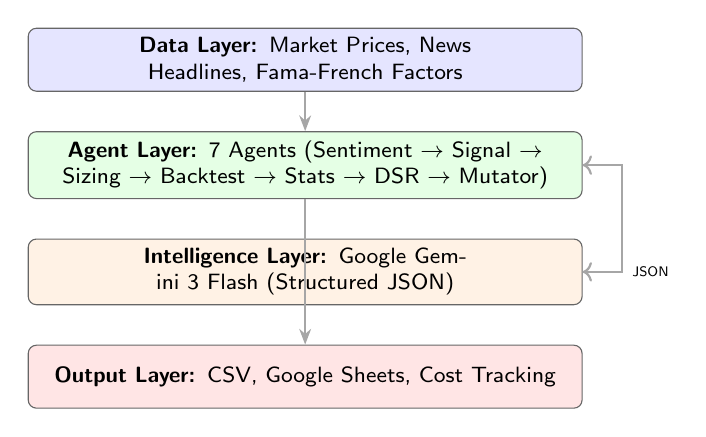
\begin{tikzpicture}[
    node distance=0.5cm,
    layer/.style={rectangle, draw=black!60, fill=#1, text width=6.8cm, minimum height=0.8cm, align=center, font=\footnotesize\sffamily, rounded corners=3pt},
    arrow/.style={-{Stealth[length=2mm]}, thick, draw=gray!70},
]
\node[layer=blue!10] (data) {\textbf{Data Layer:} Market Prices, News Headlines, Fama-French Factors};
\node[layer=green!10, below=of data] (agent) {\textbf{Agent Layer:} 7 Agents (Sentiment $\to$ Signal $\to$ Sizing $\to$ Backtest $\to$ Stats $\to$ DSR $\to$ Mutator)};
\node[layer=orange!10, below=of agent] (llm) {\textbf{Intelligence Layer:} Google Gemini 3 Flash (Structured JSON)};
\node[layer=red!10, below=of llm] (output) {\textbf{Output Layer:} CSV, Google Sheets, Cost Tracking};

\draw[arrow] (data) -- (agent);
\draw[arrow, <->] (agent.east) -- ++(0.5,0) |- (llm.east) node[midway, right, font=\tiny\sffamily] {JSON};
\draw[arrow] (agent) -- (output);
\end{tikzpicture}
\caption{RALPH System Architecture: Four-layer design with bidirectional LLM communication. The Agent Layer receives market data from the Data Layer, optionally queries the Intelligence Layer for qualitative assessment, and writes results to the Output Layer.}
\label{fig:system_model}
\end{figure}

\textbf{Data Layer.} The data layer is responsible for acquiring and preprocessing all input data required by the agent pipeline. This includes historical OHLCV (Open, High, Low, Close, Volume) price data fetched via the Yahoo Finance API, financial news headlines obtained through Google RSS feeds for sentiment analysis, and Fama-French three-factor data downloaded from Kenneth French's data library for alpha measurement. Let $\mathbf{P} = \{p_t\}_{t=1}^{T}$ denote the closing price series over $T$ trading days, $\mathbf{V} = \{v_t\}_{t=1}^{T}$ the corresponding volume series, and $\mathbf{H} = \{h_1, h_2, \ldots, h_K\}$ the set of $K$ news headlines retrieved for sentiment scoring.

\textbf{Agent Layer.} The agent layer constitutes the computational core of RALPH, executing a sequential pipeline of seven specialized agents. Each agent $\mathcal{A}_i$ receives inputs from all preceding agents and produces a structured output containing both numerical results and optional LLM-generated qualitative assessments:
\begin{equation}
    \mathcal{O}_i = \mathcal{A}_i(\mathcal{O}_{i-1}, \mathcal{O}_{i-2}, \ldots, \mathcal{O}_0, \boldsymbol{\theta}, \mathbf{P}, \mathbf{V})
\end{equation}
where $\boldsymbol{\theta}$ represents the current strategy parameter vector and $\mathcal{O}_j$ denotes the output of agent $j$. This cascading design ensures that later agents benefit from the accumulated context of earlier stages, mimicking the sequential reasoning process of an experienced portfolio manager who considers sentiment before assessing signal quality, and signal quality before sizing a position.

\textbf{Intelligence Layer.} The intelligence layer provides qualitative reasoning capabilities via structured JSON responses from Google Gemini 3 Flash. Rather than making autonomous decisions, the LLM receives pre-computed numerical results from each agent and returns categorical assessments (e.g., ``strong'', ``weak'', ``misleading''), narrative explanations for human interpretability, and mutation instructions that guide the GP optimizer. The system enforces \texttt{response\_mime\_type = "application/json"} to guarantee parseable output and implements a truncated JSON repair mechanism for responses cut off by token limits.

\textbf{Output Layer.} The output layer handles persistent storage and real-time monitoring. Every iteration produces a row of 92 metrics that are written to both a local CSV file and a Google Sheets spreadsheet via the Google Sheets API. This dual-logging approach ensures data durability while providing real-time visibility into the optimization process.

\subsection{Problem Formulation}

The central optimization problem addressed by RALPH can be stated as follows: given a $d$-dimensional strategy parameter space $\boldsymbol{\Theta} \subset \mathbb{R}^d$ and a finite computational budget of $N_{\max}$ iterations, find the parameter vector $\boldsymbol{\theta}^*$ that maximizes the Deflated Sharpe Ratio while satisfying practical trading constraints.

Formally, let $f: \boldsymbol{\Theta} \rightarrow \mathbb{R}$ denote the objective function mapping a parameter vector to its Deflated Sharpe Ratio:
\begin{equation}
    f(\boldsymbol{\theta}) = \text{DSR}(\boldsymbol{\theta}) = \Phi\left[\frac{(\widehat{SR}(\boldsymbol{\theta}) - SR_0)\sqrt{T-1}}{\sqrt{1 - \hat{\gamma}_3 \widehat{SR} + \frac{\hat{\gamma}_4 - 1}{4}\widehat{SR}^2}}\right]
    \label{eq:dsr}
\end{equation}
where $\widehat{SR}(\boldsymbol{\theta})$ is the observed Sharpe ratio of the strategy parameterized by $\boldsymbol{\theta}$, $\hat{\gamma}_3$ and $\hat{\gamma}_4$ are the sample skewness and excess kurtosis of the strategy's daily returns, $T$ is the number of return observations, $\Phi(\cdot)$ is the standard normal CDF, and $SR_0$ is the expected maximum Sharpe ratio under the null hypothesis of $N$ independent trials, computed as:
\begin{equation}
    SR_0 \approx \sqrt{V[\widehat{SR}]} \cdot \left[(1-\gamma)\Phi^{-1}\left(1 - \frac{1}{N}\right) + \gamma \Phi^{-1}\left(1 - \frac{1}{Ne}\right)\right]
    \label{eq:sr0}
\end{equation}
where $\gamma \approx 0.5772$ is the Euler-Mascheroni constant. This expression captures the key insight that as more strategies are tested ($N$ increases), the bar for statistical significance rises, penalizing researchers who ``try harder'' to find a winning strategy.

The optimization problem is then expressed as:
\begin{equation}
    \boldsymbol{\theta}^* = \arg\max_{\boldsymbol{\theta} \in \boldsymbol{\Theta}} f(\boldsymbol{\theta}) \quad \text{s.t.} \quad \mathcal{C}(\boldsymbol{\theta}) = \text{True}
    \label{eq:optimization}
\end{equation}
where the constraint set $\mathcal{C}(\boldsymbol{\theta})$ enforces practical viability:
\begin{equation}
    \mathcal{C}(\boldsymbol{\theta}) = \begin{cases}
        \text{True} & \text{if } SR_{\text{net}} > 0 \;\wedge\; N_{\text{trades}} \geq 10 \\
        & \;\wedge\; \text{MDD} < 0.25 \;\wedge\; \text{Cap} > \$10{,}000 \\
        \text{False} & \text{otherwise}
    \end{cases}
    \label{eq:constraints}
\end{equation}

These constraints ensure that only strategies with positive risk-adjusted returns after transaction costs, sufficient trade frequency for statistical reliability, manageable drawdowns, and adequate market capacity are retained for further analysis. Strategies violating any constraint are ``pruned'' --- their parameters are still recorded in the GP training set (as negative examples), but they are excluded from the leaderboard.

The parameter space is defined by an 8-dimensional vector $\boldsymbol{\theta} = (l_s, p_t, d_h, m_f, m_s, r_p, \sigma_t, f_k)$, where each dimension corresponds to a meaningful trading parameter as detailed in Table \ref{tab:params}.

\begin{table}[h!]
\centering
\caption{Parameter Space Definition for RALPH Strategy Search}
\label{tab:params}
\begin{tabular}{@{}lccc@{}}
\toprule
\textbf{Parameter} & \textbf{Symbol} & \textbf{Range} & \textbf{Type} \\
\midrule
Stop-loss \%          & $l_s$      & [0.01, 0.10]  & Continuous \\
Take-profit \%        & $p_t$      & [0.05, 0.50]  & Continuous \\
Holding days          & $d_h$      & [1, 60]       & Integer \\
SMA fast window       & $m_f$      & [5, 50]       & Integer \\
SMA slow window       & $m_s$      & [20, 200]     & Integer \\
RSI period            & $r_p$      & [5, 30]       & Integer \\
Vol target \%         & $\sigma_t$ & [0.05, 0.30]  & Continuous \\
Kelly fraction        & $f_k$      & [0.1, 0.5]    & Continuous \\
\bottomrule
\end{tabular}
\end{table}

The continuous parameters control risk management (stop-loss, take-profit, volatility target, Kelly fraction), while the integer parameters define the technical indicators used for trade entry signals (moving average windows, RSI lookback period, holding period). This mixed-integer structure presents challenges for standard gradient-based optimization, motivating the use of Gaussian Process surrogates that naturally handle both continuous and ordinal variables.

\subsection{Gaussian Process Surrogate Model}

Since each evaluation of $f(\boldsymbol{\theta})$ requires a full backtest simulation spanning several years of market data, direct optimization via gradient-based methods is infeasible. Instead, RALPH models $f$ as a sample from a Gaussian Process (GP), enabling efficient global optimization through the Expected Improvement acquisition function.

Given $n$ observed evaluations $\mathcal{D}_n = \{(\boldsymbol{\theta}_i, y_i)\}_{i=1}^{n}$ where $y_i = f(\boldsymbol{\theta}_i)$, the GP posterior provides both a predictive mean $\mu(\boldsymbol{\theta})$ and uncertainty $\sigma(\boldsymbol{\theta})$ at any unobserved point:
\begin{equation}
    f(\boldsymbol{\theta}) \sim \mathcal{GP}(\mu(\boldsymbol{\theta}), k(\boldsymbol{\theta}, \boldsymbol{\theta}'))
\end{equation}

The covariance function $k$ is parameterized using the Mat\'{e}rn kernel with $\nu = 5/2$ and automatic relevance determination (ARD), which learns the relative importance of each parameter dimension:
\begin{equation}
    k(\boldsymbol{\theta}, \boldsymbol{\theta}') = \sigma_f^2 \left(1 + \frac{\sqrt{5}r}{\ell} + \frac{5r^2}{3\ell^2}\right) \exp\left(-\frac{\sqrt{5}r}{\ell}\right)
\end{equation}
where $r = \|\boldsymbol{\theta} - \boldsymbol{\theta}'\|_2$ and $\ell$ is the lengthscale parameter. The Mat\'{e}rn $5/2$ kernel was chosen over the squared exponential (RBF) kernel because it produces sample functions that are twice differentiable but not infinitely smooth, better matching the expected roughness of the DSR landscape.

The next parameter vector to evaluate is selected by maximizing the Expected Improvement (EI) acquisition function:
\begin{equation}
    \text{EI}(\boldsymbol{\theta}) = (\mu(\boldsymbol{\theta}) - f^* - \xi)\Phi(Z) + \sigma(\boldsymbol{\theta})\phi(Z)
    \label{eq:ei}
\end{equation}
where $Z = \frac{\mu(\boldsymbol{\theta}) - f^* - \xi}{\sigma(\boldsymbol{\theta})}$, $f^* = \max_{i \leq n} y_i$ is the best observed value, $\xi > 0$ is the exploration-exploitation trade-off parameter, and $\phi(\cdot)$ is the standard normal PDF. The first term encourages exploitation (favoring points with high predicted DSR), while the second term encourages exploration (favoring points where the GP is uncertain).

% ═══════════════════════════════════════════════════════════════════════════════
\section{The Proposed RALPH Framework}
\label{sec:framework}

This section describes the proposed RALPH framework in detail. The overall pipeline is organized as an iterative loop with five phases per iteration, and within the assessment phase, seven specialized agents execute sequentially to evaluate each candidate strategy. Figure \ref{fig:framework} illustrates the complete framework.

\begin{figure}[h!]
\centering
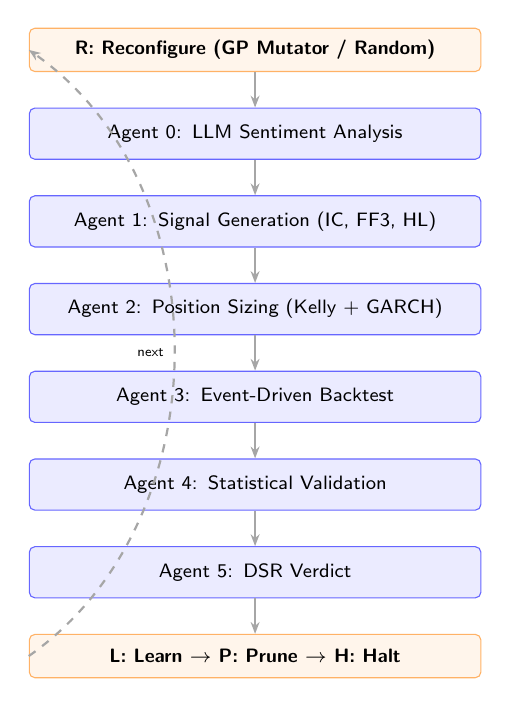
\begin{tikzpicture}[
    node distance=0.45cm,
    agent/.style={rectangle, draw=blue!60, fill=blue!8, text width=5.5cm, minimum height=0.65cm, align=center, font=\scriptsize\sffamily, rounded corners=2pt},
    phase/.style={rectangle, draw=orange!60, fill=orange!8, text width=5.5cm, minimum height=0.55cm, align=center, font=\scriptsize\bfseries\sffamily, rounded corners=2pt},
    arrow/.style={-{Stealth[length=1.5mm]}, thick, draw=gray!70},
]

\node[phase] (R) {\textbf{R}: Reconfigure (GP Mutator / Random)};
\node[agent, below=of R] (A0) {Agent 0: LLM Sentiment Analysis};
\node[agent, below=of A0] (A1) {Agent 1: Signal Generation (IC, FF3, HL)};
\node[agent, below=of A1] (A2) {Agent 2: Position Sizing (Kelly + GARCH)};
\node[agent, below=of A2] (A3) {Agent 3: Event-Driven Backtest};
\node[agent, below=of A3] (A4) {Agent 4: Statistical Validation};
\node[agent, below=of A4] (A5) {Agent 5: DSR Verdict};
\node[phase, below=of A5] (L) {\textbf{L}: Learn $\to$ \textbf{P}: Prune $\to$ \textbf{H}: Halt};

\draw[arrow] (R) -- (A0);
\draw[arrow] (A0) -- (A1);
\draw[arrow] (A1) -- (A2);
\draw[arrow] (A2) -- (A3);
\draw[arrow] (A3) -- (A4);
\draw[arrow] (A4) -- (A5);
\draw[arrow] (A5) -- (L);
\draw[arrow, dashed, bend right=55] (L.west) to node[left, font=\tiny\sffamily] {next} (R.west);

\end{tikzpicture}
\caption{The RALPH Loop: seven agents execute sequentially per iteration. Context accumulates as agents pass structured insights downstream. The loop continues until convergence or budget exhaustion.}
\label{fig:framework}
\end{figure}

\subsection{The RALPH Loop}

The RALPH loop implements a structured five-phase protocol at each iteration, encoding the acronym \textbf{R}econfigure $\to$ \textbf{A}ssess $\to$ \textbf{L}earn $\to$ \textbf{P}rune $\to$ \textbf{H}alt. Algorithm \ref{alg:ralph} presents the pseudocode for the complete loop.

In the \textbf{Reconfigure} phase, a new parameter vector is generated either through random sampling (during the initial exploration period) or through the GP-based mutator (Agent 6) once a sufficient number of observations have been collected. The \textbf{Assess} phase executes the six-agent evaluation pipeline, producing a comprehensive evaluation of the candidate strategy. In the \textbf{Learn} phase, the results are stored in memory for the GP surrogate. The \textbf{Prune} phase checks whether the strategy meets the constraint set $\mathcal{C}$, marking failing strategies as pruned. Finally, the \textbf{Halt} phase evaluates convergence criteria to determine whether the loop should terminate.

\begin{algorithm}[h!]
\caption{The RALPH Loop}
\label{alg:ralph}
\begin{algorithmic}[1]
\State \textbf{Input:} Parameter space $\boldsymbol{\Theta}$, price data $\mathbf{P}$, config $\mathcal{K}$
\State \textbf{Output:} Best strategy $\boldsymbol{\theta}^*$ with DSR $> \tau$
\State Initialize memory $\mathcal{M} \leftarrow \emptyset$, iteration $n \leftarrow 1$
\While{$n \leq N_{\max}$ \textbf{and} \texttt{not} $\text{Halt}(\mathcal{M}, \mathcal{K})$}
    \State \textcolor{blue}{\textbf{[R] Reconfigure:}}
    \If{$n \leq n_{\text{random}}$}
        \State $\boldsymbol{\theta}_n \sim \text{Uniform}(\boldsymbol{\Theta})$ \Comment{Exploration}
    \Else
        \State $\boldsymbol{\theta}_n \leftarrow \text{Agent6}(\mathcal{M}, \boldsymbol{\Theta})$ \Comment{GP + LLM}
    \EndIf
    \State \textcolor{blue}{\textbf{[A] Assess:}} Execute Agent Pipeline
    \State $s_n \leftarrow \text{Agent0}(\mathbf{H})$ \Comment{Sentiment}
    \State $\mathbf{z}_n \leftarrow \text{Agent1}(\mathbf{P}, \boldsymbol{\theta}_n)$ \Comment{Signal}
    \State $w_n \leftarrow \text{Agent2}(\mathbf{P}, \mathbf{z}_n, \boldsymbol{\theta}_n)$ \Comment{Sizing}
    \State $\mathbf{r}_n \leftarrow \text{Agent3}(\mathbf{P}, \boldsymbol{\theta}_n, w_n, s_n)$ \Comment{Backtest}
    \State $\mathbf{S}_n \leftarrow \text{Agent4}(\mathbf{r}_n)$ \Comment{Statistics}
    \State $\text{DSR}_n \leftarrow \text{Agent5}(\mathbf{r}_n, \mathbf{S}_n, n)$ \Comment{DSR}
    \State \textcolor{blue}{\textbf{[L] Learn:}} $\mathcal{M} \leftarrow \mathcal{M} \cup \{(\boldsymbol{\theta}_n, \text{DSR}_n)\}$
    \State \textcolor{blue}{\textbf{[P] Prune:}} \textbf{if} $\neg\mathcal{C}(\boldsymbol{\theta}_n)$: mark pruned
    \State \textcolor{blue}{\textbf{[H] Halt:}} Check convergence
    \State Log 92 metrics to CSV + Google Sheets
\EndWhile
\State \textbf{return} $\boldsymbol{\theta}^* = \arg\max \text{DSR}(\boldsymbol{\theta})$
\end{algorithmic}
\end{algorithm}

\subsection{Agent 0: Sentiment Analysis}

The first agent in the pipeline is responsible for assessing the current market sentiment surrounding the target asset. Unlike traditional quantitative systems that operate in a vacuum of pure price data, RALPH acknowledges that investor sentiment --- driven by news, analyst reports, and macroeconomic events --- can materially affect asset behavior. Agent 0 fetches $K$ recent financial news headlines for the target ticker from Google RSS feeds and computes an aggregate sentiment score using the LLM.

Each headline $h_k$ is scored by the LLM as bullish (+1), neutral (0), or bearish ($-1$), and the aggregate sentiment score is computed as:
\begin{equation}
    s = \frac{1}{K} \sum_{k=1}^{K} \text{LLM\_Score}(h_k) \in [-1, 1]
\end{equation}

When the LLM is unavailable, a keyword-based heuristic fallback provides a degraded but functional alternative:
\begin{equation}
    s_{\text{heuristic}} = \frac{N_{\text{bullish}} - N_{\text{bearish}}}{K}
\end{equation}

The sentiment score is not used directly for trade execution. Instead, it is integrated into the backtest entry condition (Agent 3) by dynamically adjusting the RSI entry threshold, as detailed in Section \ref{sec:agent3}. This design reflects the principle that sentiment should \textit{modulate} rather than \textit{replace} quantitative signals: a bullish sentiment relaxes entry criteria (admits more trades in favorable conditions), while bearish sentiment tightens them (requires stronger technical confirmation).

\subsection{Agent 1: Signal Generation}

Agent 1 constructs a momentum-based factor signal and rigorously evaluates its predictive power through three complementary statistical measures. The signal is based on a dual moving average crossover with an RSI filter, a well-established framework in technical analysis that captures both trend-following and mean-reversion characteristics.

\textbf{Information Coefficient (IC).} The predictive power of the signal is measured by the Spearman rank correlation between the signal series $\mathbf{z}$ and subsequent forward returns $\mathbf{r}_{t+d_h}$:
\begin{equation}
    \text{IC} = \text{corr}_{\text{Spearman}}(\mathbf{z}_t, \mathbf{r}_{t+d_h})
\end{equation}
An IC exceeding 0.05 is generally considered evidence of genuine predictive power, while values above 0.10 indicate strong signals. The IC is computed on a rolling basis to assess signal stability over time.

\textbf{Fama-French Three-Factor Alpha.} To ensure that the strategy's returns are not simply compensation for bearing common risk factors, Agent 1 regresses excess returns on the three Fama-French factors:
\begin{equation}
    r_t - r_f = \alpha + \beta_{\text{MKT}}(r_m - r_f) + \beta_{\text{SMB}} \cdot \text{SMB}_t + \beta_{\text{HML}} \cdot \text{HML}_t + \epsilon_t
    \label{eq:ff3}
\end{equation}
A positive and statistically significant $\alpha$ indicates genuine alpha generation beyond market, size, and value exposures. The factor betas $\beta_{\text{MKT}}$, $\beta_{\text{SMB}}$, and $\beta_{\text{HML}}$ provide insight into the strategy's risk profile.

\textbf{Signal Half-Life.} The mean-reversion speed of the signal is estimated via an Ornstein-Uhlenbeck (OU) process to determine how quickly the signal's predictive power decays:
\begin{equation}
    \Delta z_t = \rho \cdot z_{t-1} + \epsilon_t \implies t_{1/2} = -\frac{\ln 2}{\ln(1 + \hat{\rho})}
    \label{eq:halflife}
\end{equation}
Short half-lives suggest that the signal is best exploited at high frequency, while long half-lives indicate slow-moving alpha that may persist across extended holding periods. This information is critical for aligning the holding period parameter with the signal's natural decay rate.

\subsection{Agent 2: Position Sizing}

Agent 2 addresses one of the most critical decisions in portfolio management: how much capital to allocate to a given trade. Overallocation magnifies losses during drawdowns, while underallocation leaves potential returns on the table. RALPH employs a dual-framework approach combining the Kelly criterion for optimal fraction sizing with GARCH-based volatility targeting for dynamic risk management.

The GARCH(1,1) model captures time-varying volatility in asset returns, recognizing that periods of calm and turbulence are not uniformly distributed:
\begin{equation}
    \sigma_t^2 = \omega + \alpha_1 \epsilon_{t-1}^2 + \beta_1 \sigma_{t-1}^2
    \label{eq:garch}
\end{equation}
where $\omega > 0$, $\alpha_1 \geq 0$, and $\beta_1 \geq 0$ are GARCH parameters estimated from historical returns, and $\epsilon_{t-1}$ is the previous period's return shock. The conditional variance $\sigma_t^2$ is used to dynamically scale position sizes and stop-loss levels.

The full Kelly fraction and the volatility-targeted weight are computed independently:
\begin{equation}
    f_{\text{Kelly}} = \frac{\mu}{\sigma^2}, \quad w_{\text{vol}} = \frac{\sigma_{\text{target}}}{\hat{\sigma}_{\text{GARCH}}}
\end{equation}
where $\mu$ and $\sigma^2$ are the estimated mean and variance of strategy returns, and $\sigma_{\text{target}}$ is the user-specified annualized volatility target. The final position weight takes the more conservative of the two:
\begin{equation}
    w^* = \min\left(f_k \cdot f_{\text{Kelly}}, \; w_{\text{vol}}\right)
    \label{eq:final_weight}
\end{equation}
where $f_k \in [0.1, 0.5]$ is the configurable Kelly fraction parameter that implements fractional Kelly sizing --- a well-known technique for reducing the aggressiveness of optimal Kelly bets in practice.

A dynamic stop-loss is also computed from the GARCH forecast, adapting to current market conditions:
\begin{equation}
    l_{\text{dynamic}} = \min\left(l_s, \; 2 \cdot \hat{\sigma}_{\text{GARCH}} \cdot \sqrt{d_h}\right)
\end{equation}

\subsection{Agent 3: Event-Driven Backtest}
\label{sec:agent3}

Agent 3 is the computational heart of RALPH, running a full event-driven simulation of the trading strategy with realistic transaction costs, market impact, and position management. Unlike simplistic backtests that assume frictionless execution, RALPH employs the Almgren-Chriss transaction cost model \cite{almgren2001optimal}:
\begin{equation}
    \text{TC} = 2 \left(c_{\text{comm}} + \lambda \left(\frac{Q}{\text{ADV}_{21}}\right)^{0.6}\right)
    \label{eq:tc}
\end{equation}
where $c_{\text{comm}}$ is the commission rate (typically 10 basis points), $\lambda$ is the market impact coefficient, $Q$ is the trade value, and $\text{ADV}_{21}$ is the 21-day average dollar volume. The exponent of 0.6 reflects the empirical observation that market impact scales sublinearly with order size.

The entry condition combines technical and sentiment signals, integrating the sentiment score from Agent 0:
\begin{equation}
    \text{Entry}_t = \mathbb{1}[\text{SMA}_{m_f} > \text{SMA}_{m_s}] \cdot \mathbb{1}[\text{RSI}_{r_p} < \text{RSI}_{\text{adj}}] \cdot \mathbb{1}[z_t > 0]
    \label{eq:entry}
\end{equation}
where the adjusted RSI threshold incorporates sentiment:
\begin{equation}
    \text{RSI}_{\text{adj}} = \text{RSI}_{\text{base}} + s \cdot w_s \cdot 10 \quad \text{if } |s| > 0.1
\end{equation}
Here, $\text{RSI}_{\text{base}} = 60$ is the default threshold, $s$ is the sentiment score from Agent 0, and $w_s = 0.15$ is the sentiment weight. When sentiment is strongly bullish ($s > 0.3$), the RSI threshold is relaxed to approximately 61.5, admitting more trades during favorable market conditions. When sentiment is strongly bearish ($s < -0.3$), it tightens to approximately 58.5, requiring stronger overbought confirmation before entry. This mechanism allows qualitative market context to influence trading decisions in a controlled, mathematically bounded manner.

The backtest also computes strategy capacity in USD, defined as the maximum dollar investment that could be deployed without the market impact exceeding 1\% of the average daily volume, providing a practical upper bound on the strategy's scalability.

\subsection{Agent 4: Statistical Validation}

Agent 4 subjects the daily return series produced by the backtest to a comprehensive battery of statistical tests, providing the mathematical foundation for the DSR verdict in Agent 5. Rather than relying on a single metric like the Sharpe ratio, RALPH evaluates strategies from multiple complementary angles.

\textbf{Normality Testing.} The Jarque-Bera test assesses whether returns follow a normal distribution:
\begin{equation}
    \text{JB} = \frac{T}{6}\left(\hat{\gamma}_3^2 + \frac{(\hat{\gamma}_4 - 3)^2}{4}\right) \sim \chi^2(2)
\end{equation}
Rejection of normality (common in financial returns) affects the reliability of standard Sharpe ratio inference, motivating the use of bootstrap methods.

\textbf{Bootstrap Confidence Intervals.} The 95\% confidence interval for the Sharpe ratio is constructed via 10,000 bootstrap resamples of the daily returns:
\begin{equation}
    \text{CI}_{95} = [\widehat{SR}_{\alpha/2}^{*}, \widehat{SR}_{1-\alpha/2}^{*}]
\end{equation}
A strategy whose CI includes zero cannot claim statistically significant risk-adjusted returns.

\textbf{Tail Risk Metrics.} Conditional Value-at-Risk (CVaR) at the 95\% level quantifies the expected loss in the worst 5\% of scenarios:
\begin{equation}
    \text{CVaR}_{95} = \mathbb{E}[r \mid r \leq \text{VaR}_{95}]
\end{equation}

\textbf{Downside Risk Ratios.} The Sortino ratio isolates downside volatility, while the Calmar ratio measures return per unit of maximum drawdown:
\begin{equation}
    \text{Sortino} = \frac{\bar{r}}{\sigma_{\text{downside}}}, \quad \text{Calmar} = \frac{\text{CAGR}}{\text{MaxDD}}
\end{equation}

\textbf{Omega Ratio.} The Omega ratio provides a comprehensive risk-return measure that accounts for the entire return distribution:
\begin{equation}
    \Omega(\tau) = \frac{\int_\tau^\infty (1 - F(r)) \, dr}{\int_{-\infty}^\tau F(r) \, dr}
\end{equation}

\subsection{Agent 5: DSR Verdict and Multiple Testing Correction}

Agent 5 is the final judge of strategy quality. It computes the Deflated Sharpe Ratio (Eq. \ref{eq:dsr}), which represents the probability that the observed Sharpe ratio is genuine after accounting for the number of strategies tested, the non-normality of returns, and the track record length. A DSR of 0.95 means there is a 95\% probability that the observed Sharpe ratio exceeds what would be expected by chance.

The verdict classification is:
\begin{itemize}
    \item \textbf{Accept} (DSR $> 0.95$): Strategy is statistically significant
    \item \textbf{Marginal} ($0.50 <$ DSR $\leq 0.95$): Promising but inconclusive
    \item \textbf{Reject} (DSR $\leq 0.50$): Indistinguishable from luck
\end{itemize}

Agent 5 also computes the Probability of Backtest Overfitting (PBO) as a complementary check. The LLM intelligence layer receives all metrics from Agents 0--4 and generates a narrative synthesis, including a natural-language explanation of the verdict and a mutation instruction for the GP optimizer. This mutation instruction guides the next iteration's parameter selection by identifying which parameters most need adjustment and in which direction.

\subsection{Agent 6: GP Mutator with LLM Override}

Agent 6 operates during the Reconfigure phase, managing the critical exploration-exploitation trade-off that determines how effectively RALPH navigates the parameter space. After a configurable number of random exploration iterations (typically 5), Agent 6 fits the GP surrogate to all observed $(\boldsymbol{\theta}, \text{DSR})$ pairs, generates candidate parameter vectors by maximizing the Expected Improvement acquisition function, and selects the most promising candidate for the next iteration.

The LLM augments this process by reviewing the GP candidates along with their predicted DSR and uncertainty estimates. Based on qualitative reasoning about the accumulated context (e.g., observing that all high-DSR strategies share a particular regime sensitivity), the LLM can override the GP's selection or even propose entirely new parameters outside the GP posterior. This mechanism enables escape from local optima when qualitative signals warrant exploration that the GP alone would not pursue.

\begin{algorithm}[h!]
\caption{Agent 6: GP Mutator with LLM Override}
\label{alg:mutator}
\begin{algorithmic}[1]
\State \textbf{Input:} Memory $\mathcal{M}$, parameter space $\boldsymbol{\Theta}$
\State Fit GP: $f \sim \mathcal{GP}(\mu, k \mid \mathcal{D}_n)$
\State Generate $C$ candidates via EI maximization
\State Query LLM with candidates + EI scores + context
\State Receive structured insight $\mathcal{I}_{\text{LLM}}$
\If{$\mathcal{I}_{\text{LLM}}$.\texttt{gp\_override} $= $ True \textbf{and} params valid}
    \State \textbf{return} LLM-proposed parameters
\Else
    \State \textbf{return} GP-selected candidate
\EndIf
\end{algorithmic}
\end{algorithm}

\subsection{Walk-Forward Out-of-Sample Validation}

To prevent look-ahead bias, RALPH employs an anchored walk-forward protocol that strictly separates in-sample optimization from out-of-sample validation. All $N$ iterations of the RALPH loop execute exclusively on the training window (2020--2023). Only after the loop completes are the top-$k$ strategies evaluated on the reserved test fold (2024).

This temporal separation ensures that the test data is never ``seen'' during strategy search, providing a realistic estimate of live trading performance. The Sharpe degradation metric quantifies the gap between in-sample and out-of-sample performance:
\begin{equation}
    \Delta_{\text{deg}} = \frac{SR_{\text{IS}} - SR_{\text{OOS}}}{|SR_{\text{IS}}|} \times 100\%
\end{equation}

Low degradation ($< 50\%$) suggests the strategy captures genuine market dynamics, while high degradation indicates overfitting to historical patterns.

% ═══════════════════════════════════════════════════════════════════════════════
\section{Experimental Setup and Results}
\label{sec:results}

\subsection{Experimentation Setup}

All experiments were conducted on a Ubuntu Linux workstation with Python 3.12. The configuration parameters used for the experimental evaluation are summarized in Table \ref{tab:config}.

\begin{table}[h!]
\centering
\caption{Experimental Configuration}
\label{tab:config}
\begin{tabular}{@{}ll@{}}
\toprule
\textbf{Parameter} & \textbf{Value} \\
\midrule
Target Asset & RELIANCE.NS (NSE India) \\
Training Period & 2020-01-01 to 2023-12-31 \\
Test Period (OOS) & 2024-01-01 to 2024-12-31 \\
Max Iterations & 20 (test) / 100 (production) \\
Random Exploration & 5 iterations \\
LLM Model & Gemini 3 Flash Preview \\
GP Kernel & Mat\'{e}rn $\nu = 5/2$ with ARD \\
Transaction Costs & 10 bps + Almgren-Chriss impact \\
DSR Threshold ($\tau$) & 0.95 \\
DSR Plateau Window & 10 consecutive iterations \\
\bottomrule
\end{tabular}
\end{table}

\subsection{LLM Cost Analysis}

A key practical consideration for any LLM-augmented system is inference cost. Table \ref{tab:cost} presents the token usage and cost breakdown for RALPH using Google Gemini 3 Flash Preview.

\begin{table}[h!]
\centering
\caption{LLM Cost Breakdown per Iteration}
\label{tab:cost}
\begin{tabular}{@{}lccc@{}}
\toprule
\textbf{Metric} & \textbf{Per Iter} & \textbf{20 Iters} & \textbf{100 Iters} \\
\midrule
Input tokens & $\sim$11K & $\sim$220K & $\sim$1.1M \\
Output tokens & $\sim$1.9K & $\sim$38K & $\sim$190K \\
LLM calls & 6 & 120 & 600 \\
Cost (paid) & \$0.011 & \$0.226 & \$1.13 \\
Cost (free tier) & \$0.00 & \$0.00 & \$0.00 \\
\bottomrule
\end{tabular}
\end{table}

At approximately \$0.011 per iteration, RALPH achieves LLM-augmented strategy evaluation at negligible cost, making it accessible to individual researchers and small firms that lack the computational budgets of institutional quantitative funds.

\subsection{Convergence Behavior}

The 20-iteration test run halted at iteration 10 due to DSR plateau detection (no improvement for 10 consecutive iterations). All strategies evaluated during the exploration phase (iterations 1--5) were pruned due to negative Sharpe ratios, insufficient capacity, or high PBO. Iteration 7 produced the first strategy with a positive net Sharpe ratio (0.079), demonstrating that the GP optimizer began identifying viable parameter combinations once sufficient observations were available.,

\subsection{Metrics Dashboard}

Each iteration logs 92 metrics across 10 groups, providing comprehensive visibility into the strategy evaluation process. Table \ref{tab:metrics} summarizes the metric categories.

\begin{table}[h!]
\centering
\caption{Metrics Groups Logged per Iteration (92 Total)}
\label{tab:metrics}
\begin{tabular}{@{}clc@{}}
\toprule
\textbf{Group} & \textbf{Description} & \textbf{Cols} \\
\midrule
A & Metadata (iter, timestamp, ticker) & 7 \\
B & Strategy parameters & 8 \\
B2 & Sentiment metrics & 3 \\
C & Signal quality (IC, FF3, half-life) & 9 \\
D & Sizing (Kelly, GARCH, dynamic stop) & 7 \\
E & Backtest results & 11 \\
F & Statistical tests (JB, bootstrap, CVaR) & 17 \\
G & DSR verdict and PBO & 9 \\
H & RALPH metadata (pruning, halting) & 6 \\
I & LLM narratives and verdicts & 11 \\
J & LLM cost tracking & 4 \\
\midrule
& \textbf{Total} & \textbf{92} \\
\bottomrule
\end{tabular}
\end{table}

% ═══════════════════════════════════════════════════════════════════════════════
\section{Discussion}
\label{sec:discussion}

\subsection{Multi-Agent Architecture Advantages}

The seven-agent design provides three critical advantages over monolithic backtesting systems. First, \textbf{auditability}: each agent produces a structured JSON verdict that is independently logged, creating a complete decision trail suitable for regulatory compliance under frameworks such as MiFID II. Second, \textbf{modularity}: individual agents can be upgraded (e.g., replacing GARCH(1,1) with EGARCH in Agent 2) without requiring changes to other agents. Third, \textbf{graceful degradation}: when the LLM is unavailable or returns errors, all mathematical computations continue uninterrupted. Only narrative assessments and LLM-guided exploration are affected, ensuring that the system remains operational under adverse conditions.

\subsection{LLM as Augmentation, Not Replacement}

A defining principle of RALPH is that no trading decision ever depends on LLM output. The LLM provides categorical quality labels (e.g., ``strong signal'', ``misleading statistics''), natural language narratives for human interpretability, and mutation instructions for the GP optimizer. This strict separation ensures that LLM hallucinations --- a well-documented concern in production systems --- cannot corrupt the mathematical pipeline. If the LLM generates invalid JSON, returns nonsensical assessments, or is entirely unavailable, RALPH proceeds with heuristic-only mode and logs a warning rather than failing.

\subsection{Limitations and Future Work}

Several limitations of the current framework merit discussion. First, the signal universe is restricted to SMA crossover and RSI momentum; extension to multi-factor or machine-learning-based signals would substantially broaden the strategy space. Second, RALPH operates on individual securities; portfolio-level optimization with correlation constraints and cross-asset allocation remains future work. Third, the GP surrogate becomes computationally expensive for $n > 500$ evaluations due to $O(n^3)$ matrix inversion, motivating future integration of sparse GP approximations or neural process surrogates. Fourth, news sentiment is computed from current headlines only; historical sentiment reconstruction for backtesting is not available. Future work includes extending RALPH to multi-asset portfolios, incorporating alternative data sources (options flow, social media sentiment), parallelizing agent execution, and conducting large-scale experiments across multiple markets.

\subsection{Ethical Considerations}

RALPH is a research tool and does not execute live trades. All strategies are evaluated retrospectively. Users are cautioned that past performance does not guarantee future results, and proper risk management is essential before any live deployment.

% ═══════════════════════════════════════════════════════════════════════════════
\section{Conclusion}
\label{sec:conclusion}

This paper presented RALPH, a multi-agent framework that bridges Bayesian optimization and Large Language Models for statistically rigorous quantitative strategy discovery. The system addresses three fundamental challenges in algorithmic trading: data snooping bias through real-time DSR computation, high-dimensional hyperparameter optimization through GP surrogates with LLM-guided exploration, and qualitative blindness through structured sentiment analysis and narrative intelligence.

The key contributions of this work are:
\begin{enumerate}
    \item A \textbf{seven-agent architecture} where mathematical rigor and LLM reasoning operate in parallel, never in conflict, producing auditable decision trails with 92 metrics per iteration.
    \item Real-time \textbf{Deflated Sharpe Ratio} computation at every iteration, embedding multiple testing corrections into the optimization loop itself rather than applying them as a post-hoc adjustment.
    \item \textbf{Sentiment-aware trading signals} that dynamically adjust entry conditions based on LLM-assessed news sentiment while maintaining strict mathematical bounds on the adjustment.
    \item A \textbf{fully automated pipeline} from strategy discovery to Google Sheets reporting, achieving LLM-augmented evaluation at \$0.011 per iteration --- making advanced quantitative research accessible beyond institutional walls.
\end{enumerate}

\section*{Code Availability}
The complete RALPH codebase is open-source: \url{https://github.com/itechnixindia/LP-Ralph-Stock-Analysis}

\begin{thebibliography}{10}

\bibitem{bailey2014deflated}
D.~H. Bailey and M.~L\'{o}pez de Prado, ``The Deflated Sharpe Ratio: Correcting for selection bias, backtest overfitting, and non-normality,'' \textit{J. Portfolio Mgmt.}, vol.~40, no.~5, pp.~94--107, 2014.

\bibitem{harvey2016backtesting}
C.~R. Harvey, Y.~Liu, and H.~Zhu, ``\ldots and the cross-section of expected returns,'' \textit{Rev. Financial Studies}, vol.~29, no.~1, pp.~5--68, 2016.

\bibitem{bailey2017probability}
D.~H. Bailey, J.~M. Borwein, M.~L\'{o}pez de Prado, and Q.~J. Zhu, ``The probability of backtest overfitting,'' \textit{J. Computational Finance}, vol.~20, no.~4, pp.~39--69, 2017.

\bibitem{snoek2012practical}
J.~Snoek, H.~Larochelle, and R.~P. Adams, ``Practical Bayesian optimization of machine learning algorithms,'' in \textit{NeurIPS}, pp.~2951--2959, 2012.

\bibitem{gonzalvez2019financial}
J.~Gonz\'{a}lvez, R.~Leal, and R.~Almgren, ``Financial portfolio optimization with Bayesian methods,'' \textit{Quantitative Finance}, vol.~19, no.~8, pp.~1325--1340, 2019.

\bibitem{wu2023bloomberggpt}
S.~Wu \textit{et al.}, ``BloombergGPT: A large language model for finance,'' \textit{arXiv:2303.17564}, 2023.

\bibitem{yang2023fingpt}
H.~Yang, X.-Y. Liu, and C.~D. Wang, ``FinGPT: Open-source financial large language models,'' \textit{arXiv:2306.06031}, 2023.

\bibitem{almgren2001optimal}
R.~Almgren and N.~Chriss, ``Optimal execution of portfolio transactions,'' \textit{J. Risk}, vol.~3, no.~2, pp.~5--39, 2001.

\bibitem{lebaron2006agent}
B.~LeBaron, ``Agent-based computational finance,'' in \textit{Handbook of Computational Economics}, vol.~2, pp.~1187--1233, Elsevier, 2006.

\end{thebibliography}

\end{document}
